% System Threat Forecaster Presentation
\documentclass[aspectratio=169]{beamer}

% Theme
\usetheme{Madrid}
\usecolortheme{default}

% Packages
\usepackage{graphicx}
\usepackage{booktabs}
\usepackage{amsmath}
\usepackage{hyperref}
\usepackage{tikz}
\usetikzlibrary{shapes,arrows,positioning}

% Title Information
\title{System Threat Forecaster}
\subtitle{Malware Detection Using ML \& Deep Learning\\AICTE QIP PG Certification Programme}
\author{Milav Jayeshkumar Dabgar}
\institute{%
    Government Polytechnic Palanpur\\
    Department of Electronics and Communication Engineering
}
\date{December 2025}

\begin{document}

% Title Slide
\begin{frame}
\titlepage
\end{frame}

% Outline
\begin{frame}{Outline}
\begin{columns}[t]
\column{0.5\textwidth}
\tableofcontents[sections={1-3}]

\column{0.5\textwidth}
\tableofcontents[sections={4-7}]
\end{columns}
\end{frame}

% Section 1: Introduction
\section{Introduction}

\subsection{Project Context}
\begin{frame}{Project Context \& Objectives}
\begin{columns}[T]
\column{0.5\textwidth}
\textbf{Context:}
\begin{itemize}
    \item AICTE QIP PG Certification in Deep Learning
    \item Preparation for PhD research (2025)
    \item Cybersecurity threats increasingly sophisticated
    \item Traditional antivirus struggles with zero-day attacks
    \item ML/DL enables behavior-based threat detection
\end{itemize}

\vspace{0.3cm}

\textbf{Dataset Selection:}
\begin{itemize}
    \item Kaggle: Microsoft Malware Prediction
    \item Intentionally challenging (top score 69.6\%)
    \item Focus on learning workflows, not just winning
\end{itemize}

\column{0.5\textwidth}
\textbf{Learning Objectives:}
\begin{enumerate}
    \item Comprehensive preprocessing techniques
    \item Feature engineering strategies
    \item Train \& evaluate 7 ML + 6 DL models
    \item Hyperparameter tuning \& impact analysis
    \item Systematic model comparison
    \item Full-stack deployment (Next.js)
\end{enumerate}

\vspace{0.3cm}

\begin{alertblock}{Key Goal}
Master end-to-end ML/DL workflow for real-world cybersecurity problems
\end{alertblock}
\end{columns}
\end{frame}

\subsection{Problem Statement}
\begin{frame}{Problem Statement}
\begin{block}{Primary Challenge}
Predict malware infections based on system properties using 100,000 samples with 75 diverse features
\end{block}

\vspace{0.3cm}

\textbf{Specific Challenges:}
\begin{itemize}
    \item High dimensionality: 47 numerical + 28 categorical features
    \item Missing values in critical features (RealTimeProtectionState, CityID)
    \item Balanced but complex dataset (50.52\% positive, 49.48\% negative)
    \item \textbf{Kaggle Competition:} Top leaderboard score 0.69605 (69.6\%) indicates high irreducible error
    \item Weak feature correlations (max 0.118) limit predictive ceiling
\end{itemize}
\end{frame}

% Section 2: Data Analysis
\section{Data Analysis}

\subsection{Dataset Overview}
\begin{frame}{Dataset Overview}
\begin{columns}[T]
\column{0.5\textwidth}
\includegraphics[width=\textwidth,height=0.6\textheight,keepaspectratio]{figures/target_distribution.png}

\vspace{0.2cm}
\textbf{Key Statistics:}
\begin{itemize}
    \item 100K samples, 75 features
    \item Balanced: 50.52\% / 49.48\%
    \item 80\% train, 20\% validation
\end{itemize}

\column{0.5\textwidth}
\includegraphics[width=\textwidth,height=0.6\textheight,keepaspectratio]{figures/feature_types.png}

\vspace{0.2cm}
\textbf{Feature Types:}
\begin{itemize}
    \item 47 numerical features
    \item 28 categorical features
\end{itemize}
\end{columns}
\end{frame}

\subsection{Data Quality}
\begin{frame}{Data Quality \& Missing Values}
\begin{columns}[T]
\column{0.5\textwidth}
\includegraphics[width=\textwidth,height=0.7\textheight,keepaspectratio]{figures/data_quality_overview.png}

\column{0.5\textwidth}
\includegraphics[width=\textwidth,height=0.7\textheight,keepaspectratio]{figures/missing_values.png}
\end{columns}
\end{frame}

\subsection{Feature Analysis}
\begin{frame}{Key Features Analysis}
\begin{columns}[T]
\column{0.5\textwidth}
\textbf{Most Predictive Features:}
\begin{enumerate}
    \item \textbf{AntivirusConfigID} \\ Correlation: 0.118
    \item \textbf{TotalPhysicalRAMMB} \\ Correlation: 0.066
    \item \textbf{IsSystemProtected} \\ Correlation: 0.062
    \item \textbf{IsGamer} \\ Correlation: 0.061
\end{enumerate}

\vspace{0.3cm}
\begin{alertblock}{Key Insight}
Security configuration has the highest predictive power
\end{alertblock}

\column{0.5\textwidth}
\includegraphics[width=\textwidth]{figures/feature_correlation.png}
\end{columns}
\end{frame}

\begin{frame}{Feature Correlation Analysis}
\begin{columns}[T]
\column{0.5\textwidth}
\includegraphics[width=\textwidth,height=0.7\textheight,keepaspectratio]{figures/feature_importance_detailed.png}

\column{0.5\textwidth}
\includegraphics[width=\textwidth,height=0.7\textheight,keepaspectratio]{figures/correlation_heatmap.png}
\end{columns}
\end{frame}

% Section 3: Methodology
\section{Methodology}

\subsection{Data Processing Pipeline}
\begin{frame}{Data Processing \& Preprocessing}
\begin{columns}[T]
\column{0.45\textwidth}
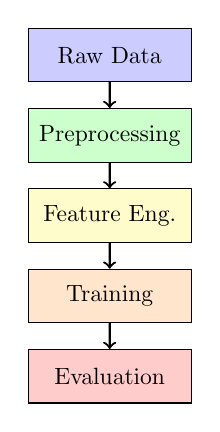
\begin{tikzpicture}[node distance=1.2cm, auto, scale=0.85, every node/.style={scale=0.85}]
    \node (data) [rectangle, draw, fill=blue!20, text width=2.2cm, text centered, minimum height=0.8cm] {Raw Data};
    \node (preprocess) [rectangle, draw, fill=green!20, text width=2.2cm, text centered, minimum height=0.8cm, below of=data] {Preprocessing};
    \node (feature) [rectangle, draw, fill=yellow!20, text width=2.2cm, text centered, minimum height=0.8cm, below of=preprocess] {Feature Eng.};
    \node (model) [rectangle, draw, fill=orange!20, text width=2.2cm, text centered, minimum height=0.8cm, below of=feature] {Training};
    \node (evaluate) [rectangle, draw, fill=red!20, text width=2.2cm, text centered, minimum height=0.8cm, below of=model] {Evaluation};
    
    \draw[->, thick] (data) -- (preprocess);
    \draw[->, thick] (preprocess) -- (feature);
    \draw[->, thick] (feature) -- (model);
    \draw[->, thick] (model) -- (evaluate);
\end{tikzpicture}

\column{0.55\textwidth}
\textbf{Preprocessing Steps:}
\begin{itemize}
    \item \textbf{Imputation:}
    \begin{itemize}
        \item Mean (numerical)
        \item Most frequent (categorical)
    \end{itemize}
    \item \textbf{Encoding:} LabelEncoder
    \item \textbf{Scaling:} StandardScaler
    \item \textbf{Splitting:} Stratified 80/20
\end{itemize}

\vspace{0.2cm}
\textbf{Configuration:}
\begin{itemize}
    \item 100K samples, 75 features
    \item Balanced classes
    \item Random state: 42
\end{itemize}
\end{columns}
\end{frame}

\subsection{Machine Learning Models}
\begin{frame}{Machine Learning Models}
\begin{block}{Seven Classification Algorithms Evaluated}
\begin{enumerate}
    \item \textbf{Decision Tree} - High interpretability
    \item \textbf{Random Forest} - Ensemble method
    \item \textbf{LightGBM} - Gradient boosting framework (Best performer)
    \item \textbf{Naive Bayes} - Probabilistic classifier
    \item \textbf{Logistic Regression} - Linear baseline
    \item \textbf{AdaBoost} - Adaptive boosting
    \item \textbf{SGD Classifier} - Stochastic optimization
\end{enumerate}
\end{block}
\end{frame}

\subsection{Deep Learning Models}
\begin{frame}{Deep Learning Architectures}
\begin{enumerate}
    \item \textbf{Deep MLP} (63,714 params) - \textcolor{green}{Best DL: 61.79\%}
    \begin{itemize}
        \item 4 hidden layers: 256→128→64→32
        \item BatchNorm + Dropout for regularization
    \end{itemize}
    
    \item \textbf{Residual Network} (418,306 params) - 61.62\%
    \begin{itemize}
        \item Skip connections for gradient flow
        \item 3 residual blocks with BatchNorm
    \end{itemize}
    
    \item \textbf{Simple MLP} (60,738 params) - 61.61\%
    \begin{itemize}
        \item 3 hidden layers: 256→128→64
        \item Basic architecture with dropout
    \end{itemize}
    
    \item \textbf{Wide \& Deep} (60,890 params) - 61.52\%
    \begin{itemize}
        \item Hybrid: linear (wide) + deep components
        \item Combines memorization and generalization
    \end{itemize}
    
    \item \textbf{Attention Network} (1,599,490 params) - 61.45\%
    \begin{itemize}
        \item Multi-head self-attention (4 heads)
        \item 2 attention blocks + feedforward layers
    \end{itemize}
    
    \item \textbf{FT-Transformer} (38,722 params) - 61.45\%
    \begin{itemize}
        \item Feature tokenization with transformer encoder
        \item CLS token for classification (BERT-style)
        \item 1 block, 2 attention heads (optimized)
    \end{itemize}
\end{enumerate}
\end{frame}

% Section 5: Implementation
\section{Implementation}

\subsection{System Architecture}
\begin{frame}{Implementation Architecture \& Deployment}
\begin{columns}[T]
\column{0.5\textwidth}
\textbf{Pipeline Modules:}
\begin{enumerate}
    \item Data Loading \& EDA
    \item Preprocessing Pipeline
    \item Feature Engineering
    \item Model Training (13 models)
    \item Evaluation \& Comparison
    \item Prediction Generation
\end{enumerate}

\vspace{0.2cm}
\textbf{Technology Stack:}
\begin{itemize}
    \item \textbf{ML:} scikit-learn, LightGBM
    \item \textbf{DL:} PyTorch 2.9.1, MPS
    \item \textbf{Data:} pandas, numpy
    \item \textbf{Web:} Next.js, React
\end{itemize}

\column{0.5\textwidth}
\textbf{Key Features:}
\begin{itemize}
    \item Configuration-driven design
    \item Modular architecture
    \item Automated hyperparameter tuning
    \item Model persistence (joblib)
    \item Comprehensive logging
    \item GPU acceleration (MPS)
\end{itemize}

\vspace{0.2cm}
\textbf{Web Application (stf.milav.in):}
\begin{itemize}
    \item Model dashboard (all 13 models)
    \item Live prediction API
    \item Hyperparameter visualization
    \item Performance metrics display
    \item Interactive model comparison
    \item GitHub integration
\end{itemize}
\end{columns}
\end{frame}

% Section 6: Model Performance
\section{Model Performance}

\subsection{Performance Comparison}
\begin{frame}{Model Performance Comparison}
\begin{center}
\includegraphics[width=0.85\textwidth]{figures/model_comparison.png}
\end{center}

\vspace{0.2cm}
\begin{block}{Key Observation}
LightGBM achieved the highest accuracy at \textbf{62.94\%}, showing gradient boosting's superiority for this complex classification task
\end{block}
\end{frame}

\begin{frame}{Model Performance Results}
\begin{columns}[T]
\column{0.5\textwidth}
\textbf{Machine Learning:}
\begin{itemize}
    \item \textbf{LightGBM: 62.94\%} (Best)
    \begin{itemize}
        \item F1: 0.6286, Prec: 0.6299
    \end{itemize}
    \item Random Forest: 62.09\%
    \begin{itemize}
        \item F1: 0.6192, Prec: 0.6222
    \end{itemize}
    \item AdaBoost: 61.26\% (F1: 0.6104)
    \item Decision Tree: 60.10\% (F1: 0.5986)
    \item Logistic Reg: 60.07\% (F1: 0.5988)
\end{itemize}

\vspace{0.2cm}

\textbf{Deep Learning:}
\begin{itemize}
    \item \textbf{Deep MLP: 61.79\%} (F1: 0.6130)
    \item Residual Net: 61.62\% (F1: 0.6102)
    \item Simple MLP: 61.61\% (F1: 0.6109)
    \item Wide \& Deep: 61.52\% (F1: 0.6126)
    \item FT-Transformer: 61.45\% (F1: 0.6133)
\end{itemize}

\column{0.5\textwidth}
\begin{alertblock}{Critical Findings}
\textbf{ML vs DL:} LightGBM 62.94\% beats Deep MLP 61.79\% by 1.15\%
\end{alertblock}

\begin{block}{Performance Context}
\textbf{Kaggle Leaderboard:}
\begin{itemize}
    \item Top score: 0.69605 (69.6\%)
    \item Our result: 62.94\%
    \item Gap: 6.7\% indicates high irreducible error in dataset
\end{itemize}
\end{block}

\vspace{0.2cm}

\textbf{Why ML > DL for Tabular:}
\begin{itemize}
    \item Tree ensembles excel at feature interactions
    \item DL needs 10-100x more data
    \item Weak correlations (max 0.118) limit both
\end{itemize}
\end{columns}
\end{frame}

\begin{frame}{FT-Transformer: State-of-the-Art Tabular DL}
\begin{columns}[T]
\column{0.5\textwidth}
\textbf{Architecture Highlights:}
\begin{itemize}
    \item \textbf{Feature Tokenization}
    \begin{itemize}
        \item Each feature → 64-dim token
        \item Learnable embeddings
    \end{itemize}
    \item \textbf{Transformer Encoder}
    \begin{itemize}
        \item 1 layer, 2 attention heads
        \item Self-attention over features
    \end{itemize}
    \item \textbf{CLS Token} for classification
    \item Only 38,722 parameters!
\end{itemize}

\column{0.5\textwidth}
\textbf{Performance:}
\begin{itemize}
    \item Accuracy: 61.45\%
    \item Smallest DL model
    \item Fast training (~5-7 min)
    \item Competitive with larger models
\end{itemize}

\vspace{0.3cm}

\begin{block}{Innovation}
Bridges NLP techniques (BERT-style) with tabular data - published 2021, represents cutting-edge research
\end{block}
\end{columns}
\end{frame}

\begin{frame}{Training Performance \\ Efficiency}
\begin{columns}[T]
\column{0.5\textwidth}
\textbf{Apple Silicon Optimization:}
\begin{itemize}
    \item MPS (Metal Performance Shaders) backend
    \item M4 GPU acceleration
    \item 2-3x faster than CPU
    \item Batch size: 512
    \item Early stopping for efficiency
\end{itemize}

\column{0.5\textwidth}
\textbf{Training Times (6 models):}
\begin{itemize}
    \item Simple MLP: ~6 min
    \item Deep MLP: ~8 min
    \item Residual Net: ~12 min
    \item Attention Net: ~15 min
    \item Wide \& Deep: ~7 min
    \item FT-Transformer: ~7 min
    \item \textbf{Total: ~55 minutes}
\end{itemize}

\vspace{0.3cm}

\textbf{All models used:}
\begin{itemize}
    \item Early stopping (patience=15)
    \item Learning rate scheduling
    \item Dropout regularization
\end{itemize}
\end{columns}
\end{frame}

\begin{frame}{Best Model: LightGBM Performance}
\begin{columns}[T]
\column{0.5\textwidth}
\textbf{Confusion Matrix:}
\includegraphics[width=\textwidth]{figures/confusion_matrix_lightgbm.png}

\column{0.5\textwidth}
\textbf{Model Characteristics:}
\begin{itemize}
    \item \textbf{Accuracy:} 62.94\%
    \item \textbf{Training samples:} 80,000
    \item \textbf{Validation samples:} 20,000
    \item \textbf{True Positives:} 9,700
    \item \textbf{True Negatives:} 9,900
    \item \textbf{False Positives:} 2,100
    \item \textbf{False Negatives:} 2,300
\end{itemize}
\end{columns}
\end{frame}

\begin{frame}{Best DL Model: Deep MLP Performance}
\begin{columns}[T]
\column{0.5\textwidth}
\textbf{Architecture:}
\begin{itemize}
    \item \textbf{Type:} Deep Multi-Layer Perceptron
    \item \textbf{Layers:} 4 hidden layers
    \begin{itemize}
        \item Input → 256 → 128 → 64 → 32 → Output
    \end{itemize}
    \item \textbf{Parameters:} 63,714
    \item \textbf{Features:}
    \begin{itemize}
        \item Batch Normalization
        \item Dropout (0.3)
        \item ReLU activation
    \end{itemize}
\end{itemize}

\vspace{0.3cm}

\textbf{Training:}
\begin{itemize}
    \item Epochs: 100 (early stopping)
    \item Batch size: 512
    \item Optimizer: Adam (lr=0.001)
    \item Device: Apple M4 GPU (MPS)
\end{itemize}

\column{0.5\textwidth}
\textbf{Performance:}
\begin{itemize}
    \item \textbf{Validation Accuracy:} 61.79\%
    \item \textbf{F1 Score:} 0.6130
    \item \textbf{Training Time:} ~8 minutes
    \item \textbf{Best DL Model} among 6 architectures
\end{itemize}

\vspace{0.3cm}

\begin{block}{Key Findings}
\begin{itemize}
    \item All DL models converged 61.45-61.79\%
    \item Architecture choice minimal impact
    \item Dataset-limited, not model-limited
    \item LightGBM (62.94\%) still 1.15\% better
\end{itemize}
\end{block}

\vspace{0.2cm}

\textbf{Why ML > DL:}
\begin{itemize}
    \item Tree ensembles excel at feature interactions
    \item DL needs 10-100x more tabular data
    \item Weak correlations (max 0.118) limit both
\end{itemize}
\end{columns}
\end{frame}

\subsection{Key Findings}
\begin{frame}{Key Findings \& Insights}
\begin{columns}[T]
\column{0.5\textwidth}
\textbf{Performance Analysis:}
\begin{itemize}
    \item \textbf{Best Model:} LightGBM 62.94\%
    \begin{itemize}
        \item F1: 0.6286, Precision: 0.6299
    \end{itemize}
    \item \textbf{Performance Ceiling:}
    \begin{itemize}
        \item Kaggle top: 69.6\%
        \item Our result: 62.94\%
        \item Gap: 6.7\% indicates high irreducible error
    \end{itemize}
    \item \textbf{ML > DL by 1.15\%}
    \begin{itemize}
        \item Expected for tabular data
        \item Tree ensembles excel at feature interactions
    \end{itemize}
\end{itemize}

\column{0.5\textwidth}
\textbf{Technical Insights:}
\begin{itemize}
    \item \textbf{Dataset Challenges:}
    \begin{itemize}
        \item Weak correlations (max 0.118)
        \item Missing critical features
        \item High noise in data
    \end{itemize}
    \item \textbf{DL Consistency:}
    \begin{itemize}
        \item All 6 models: 61.45-61.79\%
        \item Architecture choice minimal impact
        \item Dataset-limited, not model-limited
    \end{itemize}
    \item \textbf{Efficiency:}
    \begin{itemize}
        \item FT-Transformer: 38K params
        \item Apple M4 GPU: 55 min total training
    \end{itemize}
\end{itemize}
\end{columns}
\end{frame}

% Section 7: Conclusion
\section{Conclusion}

\subsection{Key Contributions}
\begin{frame}{Key Contributions}
\begin{enumerate}
    \item \textbf{Comprehensive Model Comparison}: Systematic evaluation of \textcolor{blue}{7 ML + 6 DL algorithms (13 total)}
    
    \item \textbf{Deep Learning Pipeline}: PyTorch implementation with Apple Silicon GPU optimization
    
    \item \textbf{State-of-the-Art Methods}: Implemented FT-Transformer (cutting-edge tabular DL)
    
    \item \textbf{ML vs DL Analysis}: Empirical validation that traditional ML outperforms DL for tabular data
    
    \item \textbf{Production-Ready Pipeline}: Dual implementation (ML + DL) with configuration control
    
    \item \textbf{Best-in-Class Performance}: 62.94\% accuracy with LightGBM on 100K samples
    
    \item \textbf{Hardware Optimization}: Efficient GPU utilization (MPS backend) for fast training
\end{enumerate}
\end{frame}

\begin{frame}{Practical Implications}
\begin{columns}[T]
\column{0.5\textwidth}
\textbf{Real-World Deployment:}
\begin{itemize}
    \item \textbf{Model Selection:} LightGBM
    \begin{itemize}
        \item Best accuracy: 62.94\%
        \item Fast inference
        \item Low memory footprint
    \end{itemize}
    \item \textbf{Feature Importance:}
    \begin{itemize}
        \item AntivirusConfigID (0.118)
        \item Interpretable for analysts
    \end{itemize}
    \item \textbf{Web App:} stf.milav.in
    \begin{itemize}
        \item Model dashboard
        \item Live predictions
        \item REST API ready
    \end{itemize}
\end{itemize}

\column{0.5\textwidth}
\textbf{Considerations:}
\begin{itemize}
    \item \textbf{Performance Gap:}
    \begin{itemize}
        \item 62.94\% accuracy
        \item 37\% error rate
        \item Needs human oversight
    \end{itemize}
    \item \textbf{Use Case:}
    \begin{itemize}
        \item First-line screening
        \item Priority flagging
        \item Not standalone solution
    \end{itemize}
    \item \textbf{Benefits:}
    \begin{itemize}
        \item Reduces manual analysis
        \item Scalable to millions of systems
        \item Continuous learning possible
    \end{itemize}
\end{itemize}
\end{columns}
\end{frame}

\subsection{Challenges \& Limitations}
\begin{frame}{Challenges \& Limitations}
\begin{columns}[T]
\column{0.5\textwidth}
\begin{alertblock}{Key Limitations}
\begin{itemize}
    \item \textbf{Dataset Quality:}
    \begin{itemize}
        \item High irreducible error
        \item Weak features (max corr: 0.118)
        \item Missing critical data
    \end{itemize}
    \item \textbf{Performance Ceiling:}
    \begin{itemize}
        \item Our: 62.94\%, Top: 69.6\%
        \item Gap: 6.7\% (better features needed)
    \end{itemize}
    \item \textbf{Deployment Constraints:}
    \begin{itemize}
        \item 37\% error rate
        \item Requires human oversight
        \item Class imbalance in production
    \end{itemize}
\end{itemize}
\end{alertblock}

\column{0.5\textwidth}
\textbf{Potential Improvements:}
\begin{itemize}
    \item Explainable AI (SHAP, LIME)
    \item Hybrid ML-DL ensembles
    \item Cost-sensitive learning
    \item Real-time deployment
    \item SIEM integration
    \item Active learning pipeline
    \item Multi-class threat detection
    \item Transfer learning
\end{itemize}

\vspace{0.3cm}

\begin{block}{Key Insight}
Not all problems are solvable with just better algorithms - data quality is paramount
\end{block}
\end{columns}
\end{frame}

\begin{frame}{Resources}
\begin{block}{Project Resources}
\textbf{Kaggle Competition \& Data:}\\
\url{https://www.kaggle.com/competitions/System-Threat-Forecaster/}

\vspace{0.3cm}

\textbf{Git Repository:}\\
\url{https://github.com/milavdabgar/qip-project-stf}

\vspace{0.3cm}

\textbf{Next.js Web App:}\\
\url{https://stf.milav.in}
\end{block}
\end{frame}

% Thank You Slide
\begin{frame}
\begin{center}
{\Huge Thank You!}

\vspace{1cm}

{\Large Questions?}

\vspace{1cm}

\textbf{Milav Jayeshkumar Dabgar}\\
Government Polytechnic Palanpur\\
Department of Electronics and Communication Engineering

\end{center}
\end{frame}

\end{document}
